\chapter{Test af kommunicationsprotokoler}\label{ch:test}
Dette afsnit omhandler test af de udviklede kommunikationsprotokoler. Generelt for testen af systemet gælder det, at der er blevet anvendt en bottom-up approach, hvilket betyder, at først er link-laget blevet skrevet og siden testen ved brug af minicom og mock-udgaver af transport- og applikationslaget. Det samme har været tilfældet for transportlaget, der er blevet testet ved at mocke de overliggende lag ud. I de følgende afsnit følger mere information omkring de enkelte test.

\section{Test af Link Lag}
Link laget blev testet ved at bypasse både transport og applikationslaget. Det blev gjort ved, at  applikationslaget kaldte udkritisk ned i transport laget, der siden kaldte direkte ned i link laget med dataene modtaget fra applikaionslaget.
Testen af send-metoden blev testet ved, at i den ene host blev File-clienten startet i terminalen, hvor der som argument blev givet en tekststreng med, der skulles sendes til modtageren. Modtageren blev sat op i den anden host som minicom, der blev siden verificeret, at der modtaget det rigtige på baggrund af, hvad klienten sendte. F.eks. hvis der blev sendt: "Hej"  i clienten blev der modtaget: "AHejA".


\section{Test af Transport Lag}
Det blev testet, at transportlaget kunne udføre en re-transmission ved en fejl. For at teste dette blev der introduceret en fejl i hver af metoderne send() og sendAck().Fejlen blev introduceret i begge metoder ved at smadre checksummen.
\begin{lstlisting}
	errorCount++;
	if (errorCount == 5)
	{
		buffer[0]++;
		Console.WriteLine("Fejl i transmission, forsoeger igen");
	}
\end{lstlisting}

På trods af, at fejlen blev indført virkede transmissionen, da transportlaget sørgede for re-transmission ved ødelagte data.

\section{Test af hele systemet}
Hele systemet blev testet ved at starte serveren i den ene Ubuntu Host. I den anden host blev clienten startet i terminalen, hvor den blev kaldt med sti-angivelse + filnavn på den fil, der ønskede overført. 
På billedet \ref{fig:Overforsel} ses, hvordan en test blev kørt.
\begin{figure}[H]
	\centering
	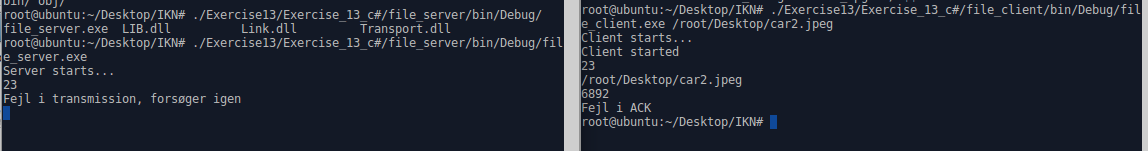
\includegraphics
	[width=140mm]{Testbilleder/overforsel.png}
	\caption{Eksempel på en overførsel}
	\label{fig:Overforsel}
\end{figure} 

Da filen var overført blev, det tjekket at den tilsendte fil var identisk med den oprindelige ved brug af den indbygge Linux kommando diff.
På figur \ref{fig:diff} ses resultatet af diff, kommandoen.
\begin{figure}[H]
	\centering
	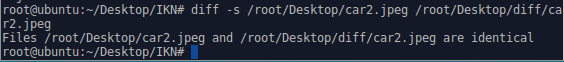
\includegraphics
	[width=140mm]{Testbilleder/diff.png}
	\caption{Ingen fejl i transmission, de to filer er identiske}
	\label{fig:diff}
\end{figure} 
Som det fremgår er den originale fil identisk med den tilsendte fil. Protokolen blev testet med flere filer, hvor den største var et billede på 5.2mb. På baggrund af disse test kunne det konkluderes at protokolstakken virkede.
